% template.tex, dated April 5 2013
% This is a template file for Annual Reviews 1 column Journals
%
% Compilation using ar-1col.cls' - version 1.0, Aptara Inc.
% (c) 2013 AR
%
% Steps to compile: latex latex latex
%
% For tracking purposes => this is v1.0 - Apr. 2013
\documentclass{ar-1col}
\usepackage{natbib}

\setcounter{secnumdepth}{4}
\usepackage{url}

% preferred fontsize
\newcommand{\mysize}{\fontsize{12}{14}\selectfont}

% Metadata Information
\jname{Xxxx. Xxx. Xxx. Xxx.}
\jvol{AA}
\jyear{YYYY}
\doi{10.1146/((please add article doi))}


% Document starts
\begin{document}

% Page header
\markboth{Ho}{Composite SED Clustering}

% Title
\title{Composite Spectral Energy Distribution and Bayesian Machine Learning for Spectral Data}

%Authors, affiliations address.
\author{Ming-Feng Ho$^1$
\affil{$^1$Department of Physics and Astronomy, University of California, Riverside; email: mho026@ucr.edu}}

%Abstract
\begin{abstract}

    
Composite SEDs and Bayesian non-parametric clustering.

Photometry and medium bands: surveys
Spectral Energy Distributions: fitting template, FAST, EAZY
Composite SEDs: evolution from grouping methods
Bayesian non-parametric on functional data:
1. Dirichlet Processes for clustering
2. Gaussian Processes on Spectral data
3. Clustering on functional data 

\end{abstract}

%Keywords, etc.
\begin{keywords}
galaxies: evolution, methods: data analysis, methods: Bayesian non-parametric
\end{keywords}
\maketitle

%Table of Contents
\tableofcontents


% Heading 1
\section{INTRODUCTION}
improvement of Photometry data on redshift rage 3-4.


% Heading 2
\section{GALAXY EVOLUTION IN TERMS OF COMPOSITE SPECTRAL ENERGY DISTRIBUTIONS (SEDs)}

% Heading 2.1
\subsection{Medium-Band Photometry}
This is dummy text. 

% Heading 2.2
\subsection{Composite Spectral Energy Distributions (SEDs)}

% Heading 3
\section{BAYESIAN MACHINE LEARNING FOR CLUSTERING AND MODELING SPECTRAL DATA}

Bayesian machine learning is a branch of machine learning which aims to solve machine learning problems in a Bayesian perspective. 
Instead of optimizing the parameters of interest from data using an empirical loss function (e.g., a least-squared function), Bayesian methods build generative models to randomly sample data from parameters and try to maximize the likelihood between observed data and hidden parameters \citep{Barber2012}.

The difference between Bayesian statistics and Bayesian ``machine learning'' is that Bayesian ``machine learning'' is trying to approximate {\it non-linear} functions \citep{Bishop2003}. 
After the publish of \citet{Rasmussen2005}, learning unknown complicated functions from observed data using {\it Gaussian processes} (\textsc{gp}) became popular. 

% Heading 3.1
\subsection{Modeling Spectral Data using Gaussian Processes (\textsc{gp})}

A {\it Gaussian process} is a bunch of random variables, and any finite subset of these random variables is a joint Gaussian distribution \citep{Rasmussen2005}. \textsc{gp} could be a powerful tool to model any kind of functional data (continuous data) in a non-parametric way. 
By non-parametric, it actually means we use infinite many parameters to describe our function \citep{Gelman04}. \textsc{gp} could be treated as a random function (or a stochastic process) which draws samples from the n-dimensional distribution, 

% draw samples from a GP
\begin{equation}
    \mu(x_1), ..., \mu(x_n) \sim Normal((m(x_1), ..., m(x_n)), K(x_1, ..., x_n)).
    \label{eq:GP}
\end{equation}

% marginal note: GP
\begin{marginnote}[120pt]
    \entry{GP}: \textit{Gaussian Processes}
    \entry{$\sim$ Normal}: Sampling from a Gaussian (normal) distribution
    \entry{Bayesian ML}: Bayesian Machine Learning    
    \entry{K}: Covariance function (matrix)
    \entry{$\mu$}: Mean function
\end{marginnote} 

The construction of a \textsc{gp} could be considered as finding the mean function ($m(\vec x)$) and a suitable covariance function ($K(\vec x, \vec x')$). 
In normal cases, a zero mean is usually used as a prior for \textsc{gp} regressions. For $K(\vec x, \vec x')$, pre-defined covariance functions (e.g., squared potential function $\exp{(\frac{-r^2}{2 \ell^2})}$) are often been implemented. 
However, the usage of \textsc{gp} in modeling functional data will also be restricted by the intrinsic properties of the covariance functions.
Learning a suitable covariance function is the most crucial part of machine learning in \textsc{gp}.

Finding a suitable choice of covariance often reflects our interpretations of the characteristics of our data  \citep{Rasmussen2005}. 
For example, the usage of the squared potential function $\exp{(\frac{-r^2}{2 \ell^2})}$ implies the assumption that we believe each point on the function would have less impact to each other if they are far away on the functional space.
Therefore, we need a special kind of covariance function to suit our purpose of modeling spctral data.

\citet{Garnett17} took a machine learning approach to learn the covariance function, with a wavelength range from Ly$_\infty$ to Ly$\alpha$, from training data (quasar spectra). 
The optimization choice was to firstly decompose covariance matrix with \citep{Garnett2015},

% decomposition of covariance
\begin{equation}
    \mathbf{K} = \mathbf{M}\mathbf{M}^{T},
    \label{eq:decompose}
\end{equation}
and then use the first 10 principle components of the flux of quasar spectra, $\mathbf{Y}$, to constitute the matrix $\mathbf{M}$. 
The optimization was done by maximizing the log likelihood, $\mathcal{L}$, of the data by given $\mathbf{M}$ and absorption noise $\omega$, 

% log likelihood
\begin{equation}
    \mathcal{L}(\mathbf{M}, \omega) = \log{ p(\mathbf{Y} \mid \mathbf{\lambda}, \mathbf{\mu}, \mathbf{M}, \mathbf{N}, \omega, z_\mathrm{qso}, Model) }.
\end{equation}

The goal of optimizing above function is to find optimal covariance matrix, $\mathbf{M}$, and absorption parameter, $\omega$, with some given conditions. Those conditions are: a given mean vector $\mathbf{\mu}$, the noise on the spectra $\mathbf{N}$, the redshift of the \textsc{qso}, and with a given model. 
In a perspective of generative modeling, optimizing the data likelihood implies we are trying to find a covariance matrix to better generate our spectral data. 

% covariance for DLA
\begin{figure}
    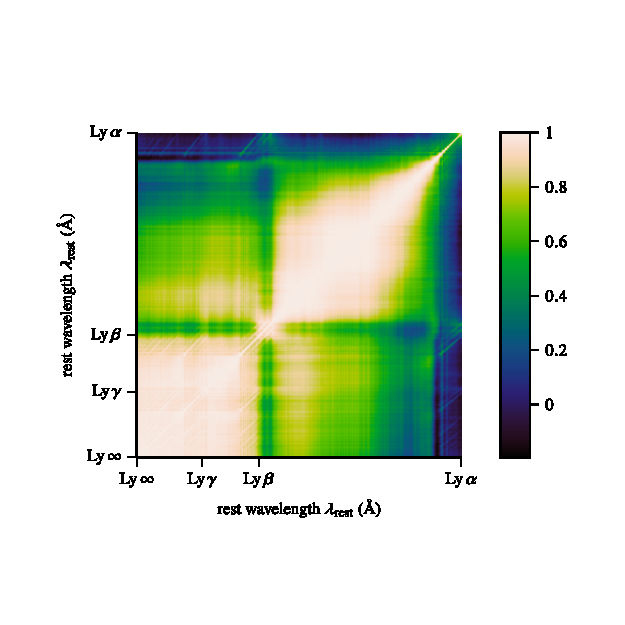
\includegraphics[width=5in, height=5in]{images/covariance.pdf}
    \caption{Covariance function for quasar spectra in \citet{Garnett17}}
    \label{fig:covariance}
\end{figure}

The covariance matrix built in \citet{Garnett17} with a wavelength range from Ly$_\infty$ to Ly$\alpha$ is in Fig~\ref{fig:covariance}. 
The scale in Fig\ref{fig:covariance} represents the strength of correlations between pairs of rest-frame wavelengths on the \textsc{qso} spectra.
The features of Lyman series are distinct.
The off-diagonal term demonstrates the correlations of pairs of corresponding emission lines.

The mean function of \textsc{gp} modeling in \citet{Garnett17} can be simply obtained by stacking the training spectra, 

% stacking QSO spectra
\begin{equation}
    \mu_j = \mathrm{median } (y_{ij}),
\end{equation}
where $y_{ij}$ are the fluxes for spectrum. Fig~\ref{fig:mean_function} shows the mean function with a range from Ly$_\infty$ to Ly$\alpha$. 
The features emission line of Lyman series are also visible in the figure.

Generally, the \textsc{gp} model for spectral data could be described as
% full model for spectral gaussian process
\begin{equation}
    p( \mathbf{y} \mid \mathbf{\lambda}, \mathbf{v}, \mathbf{\omega}, z, Model ) 
    = Normal( \mathbf{y}; \mathbf{\mu}, \mathbf{K} + \mathbf{\Omega} + \mathbf{V} ), 
\end{equation}
where $\mathbf{y}$ is the observed flux of the spectrum, 
$\mathbf{\lambda}$ is the spectroscopic grids we chose to bin the flux, 
$\mathbf{v}$ is the instrumental noise given by the observed data (it is \textsc{sdss} \textsc{qso} catalogue \citep{SDSS09} in \citet{Garnett17}), $z$ is the redshift dependence of the \textsc{gp} model, and $\omega$ is the absorption redshift dependence (it was used to model
 Ly$\alpha$ forest in \citet{Garnett17}). 
 
 The beauty of generative modeling the spectrum using \textsc{gp} framework is that we are able to fully control the modeling of instrumental noise and redshift dependence uncertainties. 
 In addition, the whole framework is transparent and flexible, which implies it is interpretable and future improvements are achievable. 


% mean function for DLA
\begin{figure}
    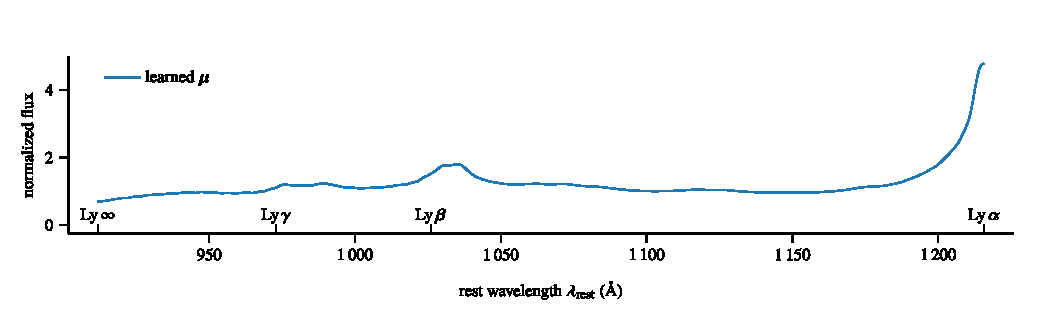
\includegraphics[width=5in, height=1.5in]{images/mean_function.pdf}
    \caption{Mean function for quasar spectra in \citet{Garnett17}}
    \label{fig:mean_function}
\end{figure}


% GP summary Points
\begin{summary}[SUMMARY POINTS]
    \begin{enumerate}
    \item \textit{Gaussian Processes}. A flexible Bayesian non-parametric framework which allows us to model any kind of function.
    \item Learned covariance matrix $\mathbf{K}$. To model spectral data, we can optimize the covariance matrix using training data to acquire customized covariance function of any given range of wavelengths.
    \end{enumerate}
\end{summary}
    

% Heading 3.2
\subsection{Dirichlet Processes}

The \textit{Dirichlet process} \citep{Teh2006} is a Bayesian non-parametric method to model infinite mixture models and also could be used for clustering. We haven't seen any application of \textit{Dirichlet processes} (\textsc{dp}) in spctral data clustering. 
A recent astronomical application of \textsc{dp} is building a mixture model for binary neutron stars in gravitational-wave data \citep{Pozzo2018}. 
Since we expect the application of \textsc{dp} in the clustering of spectral data is achievable in future, we decided to roughly review the basic concept of \textsc{dp} here.

The \textsc{dp} is a stochastic process which is often used to model mixture models. 
Each random sample in \textsc{dp} is itself a distribution, which means we can treat random samples of a \textsc{dp} as cluster centers of a mixture model. 
Similar to \textsc{gp}, a finite subset of a \textsc{dp} could be described by Dirichlet distributions.

To model the data $v$ using the Dirichlet mixture model,
the clustering memberships could be described by the following conditional probability \citep{Barber2012}, 

% indicator model
\begin{equation}
    p(v^{1:N} \mid \theta) = \sum_{z^{1:N}} p(v^{1:N} \mid z^{1:N}, \theta) p(z^{1:N}),
    \label{eq:indicator}
\end{equation}
where $p(z^{1:N})$ gives the priors over each cluster and $\theta$ describe the parameters of the cluster model. 
The choice of priors over clusters ($p(z^{1:N})$) is crucial


% Dirichlet PGM
\begin{figure}
    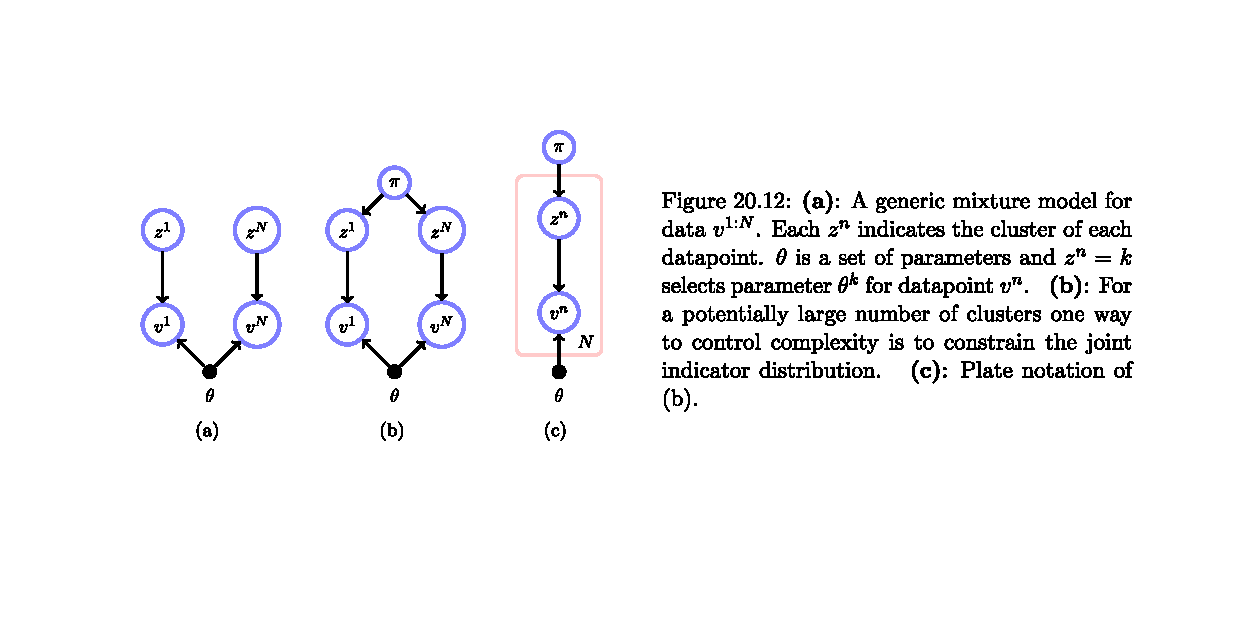
\includegraphics[width=6in, height=3in]{images/Dirichlet.pdf}
    \caption{The probabilistic graphical model of \textsc{dp} in plate notation in \citet{Barber2012}. The symbols here: $z$ is the indicator and $p(z^n)$ implies the prior over $n^{th}$ cluster; $v$ is data; $\theta$ is used to describe the parameters on the cluster model (the shared model) while $z$ could be treated as the hidden variable used to described component models (the individual models); $\pi$ here is the parameter of a Dirichlet distribution, which is used to describe distributions.}
    \label{fig:Dirichlet}
\end{figure}


% Heading 3.2.1
\subsubsection{Chinese Restaurant Process}

The clustering property of \textsc{dp} is hard to understand simply via mathematical forms above. 
However, there's an intuitive metaphor described in \citet{Teh2006} to mimic the process of drawing samples from \textsc{dp} using a real-life example: \textit{Chinese Restaurant process} (\textsc{crp}).

The name of \textsc{crp} was developed in 1980's. \textsc{crp} is a process to describe the distribution over partitions.

Now, imagine this: there are infinite number of round tables in a Chinese restaurant, and there are also infinite number of seats in each round table. 
Each customer will come to the restaurant one by one (just like sampling). 
Let's assume the first customer choose the first table.
Which table would be next person choose?


% figure: chinese restaurant
\begin{figure}
    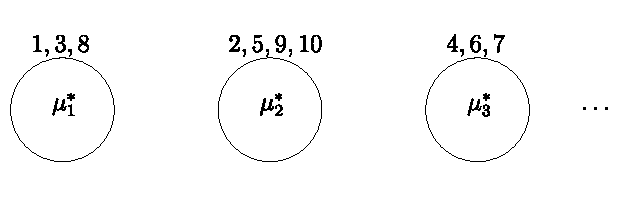
\includegraphics[width=3in, height=1in]{images/chinese_restaurant.pdf}
    \caption{An illustration of \textsc{crp} in \citet{Blei2007}.}
    \label{fig:crp}
\end{figure}

% Summary Points
\begin{summary}[SUMMARY POINTS]
\begin{enumerate}
\item Summary point 1. These should be full sentences.
\end{enumerate}
\end{summary}

% Future Issues
\begin{issues}[FUTURE ISSUES]
\begin{enumerate}
\item Future issue 1. These should be full sentences.
\end{enumerate}
\end{issues}

%Disclosure
% \section*{DISCLOSURE STATEMENT}
% If the authors have noting to disclose, the following statement will be used: The authors are not aware of any affiliations, memberships, funding, or financial holdings that
% might be perceived as affecting the objectivity of this review. 
 
% Acknowledgements
\section*{ACKNOWLEDGMENTS}
Acknowledgements, general annotations, funding.

% References
\bibliographystyle{ar-style2}
\bibliography{sample}
% \begin{thebibliography}{00}

% \bibitem[Acevedo \& Fitzjarrald(2001)]{Acevedo:01}
% Acevedo O, Fitzjarrald D. 2001.
% \textit{J. Atmos. Sci.} 58:2650--67


% \end{thebibliography}


\end{document}
